\chapter{Euler Graphs and Hamilton Graphs}

\begin{descr}
    TODO
\end{descr}

\section{Euler Graphs}\index{Euler Graphs}
\subsection{Euler 1736: K�nigsberger Br�ckenproblem}
Is it possible to do a round walk crossing every bridge exactly once?\\
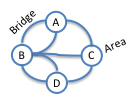
\includegraphics{diagrams/koenigsberg.png}

\begin{example}
    
\includegraphics{diagrams/haus_vom_nikolaus.png}    
\end{example}

\begin{definition}
Let $G$ be a finite undirected graph. A path $e_{1}..e_{t}$ is called a \deftxt{euler path}
if every edge in $E$ occurs exactly once in the list.\\
A graph is a \deftxt{euler graph} if it has a euler path.
\end{definition}

\begin{theorem}
    A finite connected graph is a euler graph if and only if:
    \begin{enumerate}
        \item It ha eiter exactly two nodes of odd degree.
        or
        \item All nodes have even degree.
    \end{enumerate}
\end{theorem}

In the last case the path is a cycle. In the first case no euler path is a cycle.
Check is possible in linear time.

\begin{prooof}
    $">"$ Let $G=(V,E)$ be a graph that has a euler path that is not a cycle. Let $\mid E \mid=k$
    $\circ  \xrightarrow{e_{1}} \circ \xrightarrow{e_{2}} ... \circ \xrightarrow{e_{k}}$
    In this path $v_{1}$ and $v_{k+1}$ have od degreee and all other nodes have even degree. 
    Now consider the case teht $G$ has a euler cycle.\\
    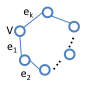
\includegraphics{diagrams/proof21.png} \\
    Hence every node has even degree. \\[2mm]
    
    $"<"$ Let $G$ be a graph with exactly two nodes with odd degree, let this be $a$ and $b$.
    We contradict a euler path as follows:\\
    Start at node $a$ and folow an edge ?inktt? on a. $a\circ  \xrightarrow{} \circ \xrightarrow{} ... \circ b$ \\
    Case 1: All edges have been used -> done \\
    Case 2: Still edges unused. Then because $G$ is connected there must be some node $v$ on 
    the path from which there is an unused edge. We construct a path starting from $v$ as before. This path must end in $v$.\\
    $\Rightarrow$ Repeat until there are no more unused edges.\\
    Analogously we proceed when the degree of all nodes is even.\\
    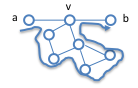
\includegraphics{diagrams/proof212.png} \\
\end{prooof}

\begin{example*}
    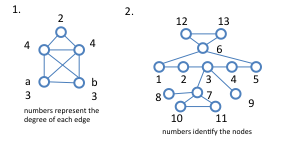
\includegraphics{diagrams/examples21.png} \\ 
\end{example*}

In the directed case a \deftxt{directed Euler path} is a directed path on which every edge appears exactly once.
Directed \deftxt{Euler cycle} analogously.\\

\begin{theorem}
    A finite directed graph is a \deftxt{directed Euler graph} if and only if its underlying undirected graph is connected.
    \begin{enumerate}
       \item There is one node $a$ with $g_{out}(a) = g_{in}(a) + 1$ and another node $b g_{out}(b) = g_{in}(b) + 1$ and
             for all other nodes $v g_{in}(v) = g_{out}(v)$. Or
       \item For all nodes $g_{in}(v) = g_{out}(v)$ (\deftxt{directed Euler cyle})
             
    \end{enumerate}
\end{theorem}


\section{Hamiltonian Graphs}\index{Hamiltonian Graphs}
\begin{definition}
    Let $G=(V,E)$ be a graph. A \deftxt{Hamiltonian cycle} $C$ is a cycle on which every node $\in V$ occurs exactly once.
    If $G$ has a Hamiltonian cycle it is called  \deftxt{Hamiltonian}.
\end{definition}
\begin{example*}
    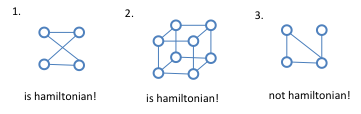
\includegraphics{diagrams/examples22.png} \\ 
\end{example*}


The problem, given an arbitrary undirected graph: Is it \deftxt{Hamiltonian}? $\Rightarrow$ NP complete $\Rightarrow$ no polinomial
time algorithm is known and it is assumed there is no such.\\
One way out of the complexity issue is to derive conditions that can be tested explicitly and if they are satisfied
the desired property is ensured.

\begin{theorem}
    Let $G=(V,E)$ be an undirected finite graph without loops and without parallel edges. Let $\left| V \right|=n$. If for all
    $x,y \in V with x \neq y$ and no edge with end points $x,y$ the following holds: \\
    $deg(x) + deg(v) \geq \left| V \right|=n$ \\
    Then $G$ has a \deftxt{Hamiltonian Cycle}.
\end{theorem}

\begin{example*}
     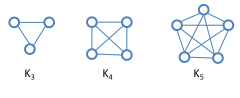
\includegraphics{diagrams/examples23.png} \\ 
\end{example*}
    
\begin{prooof}
    Assume there is a graph $G=(V,E)$ with $deg(x) + deg(y) \geq \left| V \right|$ for all $x$ and $y$ with $x \neq y$
    and no edges between them, but is not \deftxt{Hamiltonian}. Among all graphs with nodes in $V$, we choose one that
    has this property and has the maximal number of edges, we call graph $G_{0}=(V,E_{0})$. As the complete graph
    (every node is connected with every other node) is \deftxt{Hamiltonian}, we know there must be an edge $e$ connecting some $x$ 
    and $y$ and $e \in E_{0}$. \\
    We add edge $e$ to the graph and obtain a new graph $G_{1}=(V,E_{1})$ that still satisfies the degree conditions and must be \deftxt{Hamiltonian}
    because $G_{0}$ was the one with the largest number of edges.\\
    We know that the \deftxt{Hamiltonian cycle} must contain the edge $e$. \\
    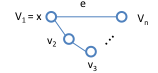
\includegraphics{diagrams/proof23.png} \\ 
    $v_{i} \neq v_{j} for i \neq j$
    
    $S = \{ v_{i}: 1 \leq i \leq n$ x,y are connected with an edge in $E_{0}\}$ \\
    $T = \{ v_{i}: 1 \leq i \leq n $ there is an edge between $y$ and $v_{i}$ in $E_{0}\}$ \\
    
    Observation:
    \begin{enumerate}
        \item $y = v_{n} \in S \cup T$
        \item $\left| S \cup T \right| < \left| V \right| = n$
        \item $deg(x) = \left| S \right|$ \\
              $deg(y) = \left| T \right|$
    \end{enumerate}
    Hence $S \cap T \neq \emptyset, let v_{j} \in S \cap T$ hence there is an edge between $x,v_{j+1}$ and an edge between $y,v_{j}$. Now remove
    edge $e$ and there is a Hamiltonian left. \\
    Cost of checking the condition $O(M^2) \left| E \right| \leq \left| V \right|^2$ \\
    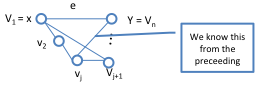
\includegraphics{diagrams/observation23.png} \\ 
\end{prooof}

\section{Bipartite Graphs}\index{Bipartite Graphs}

\begin{example*} 
    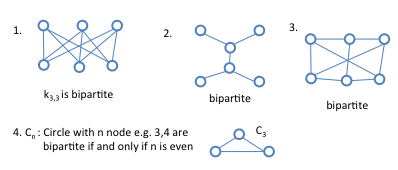
\includegraphics{diagrams/bipartiteexp.png} 
\end{example*}

\begin{theorem}
    Let $G=(V,E)$ be a connected undirected graph without loops and parallel edges. 
    $G$ is bipartite if and only if it does not contain any circle of odd length.
\end{theorem}

Corollary: All trees are bipartite

\begin{prooof}
    $\Rightarrow$ IF $G$ contains a cicle of odd length then it is not bipartite.
    $\Leftarrow$ Let $G$ not have any circle of odd length we choose node v.\\
    $V_{1} = \{ u \in V \text{a shortest path between u and v is of odd length} \}$ \\
    $V_{2} = \{ u \in V \text{a shortest path between u and v is of even length} \}$ \\
    $V \in V_{2}, V = V_{1} \dot{\cup} V_{2}$ (disjoint union) \\
    Claim: Ther is no edge $e$ with both endpoints in $V_{1}$ respectively $V_{2}$. Assume there is an edge $e$ with both
    endpoints in $V_{1}$. Let the end points be $x,y$ \\
    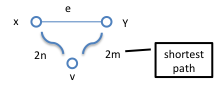
\includegraphics{diagrams/proof24.png} \\
    $2m \leq 2n + 1 \text{and} 2n \leq 2m + 1 \Rightarrow m = n$ \\
    
    Let $P(x)$ a shortest path from $v$ to $x$, analogously $P(y)$ let $w$ be the last node on the paths starting at $v$ that lies
    on both paths.
    
    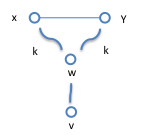
\includegraphics{diagrams/proof242.png} \\
    The length of the path from $w$ to x coincides with the length of path from $w$ to $y$. \\
    The circle w - x - y - w is of odd length i.e. $2k+1 \Rightarrow$ contradiction!
\end{prooof}

Corollary 2.5: A bipartie graph with an odd number of nodes cannot be \deftxt{Hamiltionian}

\begin{prooof}
    Assume if were Hamiltionian then there is a cycle where node appears exactly once. 
    This cycle is of odd length $\Rightarrow$ contradicts Theorem 2.4
\end{prooof}
    
\begin{example}
    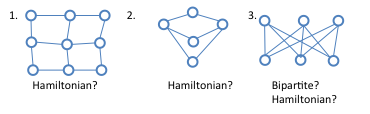
\includegraphics{diagrams/example25.png} \\
    $\Rightarrow$ We have two theorems to check:
    \begin{enumerate}
        \item Count degrees
        \item Corollary 2.5
    \end{enumerate}
\end{example}


